\documentclass[12pt, letterpaper]{article}
\usepackage[a4paper,left=3cm,right=2cm,top=2.5cm,bottom=2.5cm]{geometry}

\usepackage[utf8]{inputenc}
\usepackage{graphicx}
\graphicspath{ {images/} }
\usepackage{amsmath,bm}
\usepackage{listings}
\usepackage{float}
\usepackage{pdfpages}
\usepackage{siunitx}
\usepackage{subfig}


\title{4TN4 Assignment 3}
\author{Adam Bujak (400113347)}
\date{February 13, 2022}

\begin{document}

\maketitle

\section{Theory}

\subsection{Edge Detection, Sobel Operator}

\textbf{Sobel operators are masks used to calculate approximations of the derivative in the x-direction and y-direction. Apply the Sobel operators to the given image. Approximate magnitude and phase of the gradient at each pixel position. (Zero-Padding is NOT required for this question)}

\begin{table}[!ht]
    \centering
    \begin{tabular}{|l|l|l|l|l|l|l|l|l|l|l|l|}
    \hline
        0 & 0 & 0 & 0 & 0 & 0 & 0 & 0 & 0 & 0 & 0 & 0  \\ \hline
        0 & 0 & 0 & 0 & 0 & 0 & 0 & 0 & 0 & 0 & 0 & 0  \\ \hline
        0 & 0 & 0 & 1 & 1 & 1 & 1 & 1 & 1 & 1 & 0 & 0  \\ \hline
        0 & 0 & 0 & 0 & 1 & 1 & 1 & 1 & 1 & 1 & 0 & 0  \\ \hline
        0 & 0 & 0 & 0 & 0 & 1 & 1 & 1 & 1 & 1 & 0 & 0  \\ \hline
        0 & 0 & 0 & 0 & 0 & 0 & 1 & 1 & 1 & 1 & 0 & 0  \\ \hline
        0 & 0 & 1 & 0 & 0 & 0 & 0 & 1 & 1 & 1 & 0 & 0  \\ \hline
        0 & 0 & 0 & 1 & 0 & 0 & 0 & 0 & 1 & 1 & 0 & 0  \\ \hline
        0 & 0 & 0 & 0 & 1 & 0 & 0 & 0 & 0 & 1 & 0 & 0  \\ \hline
        0 & 0 & 0 & 0 & 0 & 1 & 0 & 0 & 0 & 0 & 0 & 0  \\ \hline
        0 & 0 & 0 & 0 & 0 & 0 & 0 & 0 & 0 & 0 & 0 & 0  \\ \hline
        0 & 0 & 0 & 0 & 0 & 0 & 0 & 0 & 0 & 0 & 0 & 0 \\ \hline
    \end{tabular}
\end{table}

To calculate the magnitude of the phase of the gradient at each pixel position we can calculate the gradient in the x and y directions and then apply the following formulas to get the phase, and magnitude:

\[ |\nabla G| = \sqrt{G_x^2 + G_y^2} \]
\[ \phi = atan2(G_y, G_x) \]

\noindent (atan2 offers easier application than the simpler phase calculation: $\phi = atan(G_y/G_x)$) when using not doing calculations by hand\\

\noindent To get $G_x$ and $G_y$ at each pixel we convolve the image at the desired pixel with the horizontal (Figure \ref{fig:x-sobel}) and vertical (Figure \ref{fig:y-sobel}) Sobel Filter kernels respectively.\\

\begin{figure}[H]
    \centering
    $\begin{bmatrix}
    -1&0&1\\
    -2&0&2\\
    -1&0&1\\
    \end{bmatrix}$
    \caption{Horizontal Sobel Filter (x-direction)}
    \label{fig:x-sobel}
\end{figure}

\begin{figure}[H]
    \centering
    $\begin{bmatrix}
    1&2&1\\
    0&0&0\\
    -1&-2&-1\\
    \end{bmatrix}$
    \caption{Vertical Sobel Filter (y-direction)}
    \label{fig:q1}
\end{figure}

For example, the calculation of convolution of the Sobel operator in the x-direction and the image at pixel [3,2] ([x,y] with indices starting at 1) would look like this:

\[ G_x = \begin{bmatrix}-1&0&1\\-2&0&2\\-1&0&-1\\\end{bmatrix} * I \]
\[ G_x(3,2) = \begin{bmatrix}-1&0&1\\-2&0&2\\-1&0&-1\\\end{bmatrix} * I(3,2) \]
\[ G_x(3,2) = \begin{bmatrix}-1&0&1\\-2&0&2\\-1&0&-1\\\end{bmatrix} \cdot \begin{bmatrix}0&0&0\\0&0&0\\0&0&1\\\end{bmatrix} \]
\[ G_x(3,2) = -1 \]

where $I$ is the image.

Doing this for all pixels in the image, we get the following image for $G_x$:

\begin{table}[H]
    \centering
    \begin{tabular}{|l|l|l|l|l|l|l|l|l|l|l|l|}
    \hline
        0 & 0 & 0 & 0 & 0 & 0 & 0 & 0 & 0 & 0 & 0 & 0  \\ \hline
        0 & 0 & -1 & -1 & 0 & 0 & 0 & 0 & 0 & 1 & 1 & 0  \\ \hline
        0 & 0 & -2 & -3 & -1 & 0 & 0 & 0 & 0 & 3 & 3 & 0  \\ \hline
        0 & 0 & -1 & -3 & -3 & -1 & 0 & 0 & 0 & 4 & 4 & 0  \\ \hline
        0 & 0 & 0 & -1 & -3 & -3 & -1 & 0 & 0 & 4 & 4 & 0  \\ \hline
        0 & -1 & 0 & 1 & -1 & -3 & -3 & -1 & 0 & 4 & 4 & 0  \\ \hline
        0 & -2 & -1 & 2 & 1 & -1 & -3 & -3 & -1 & 4 & 4 & 0  \\ \hline
        0 & -1 & -2 & 0 & 2 & 1 & -1 & -3 & -3 & 3 & 4 & 0  \\ \hline
        0 & 0 & -1 & -2 & 0 & 2 & 1 & -1 & -3 & 1 & 3 & 0  \\ \hline
        0 & 0 & 0 & -1 & -2 & 1 & 2 & 0 & -1 & 0 & 1 & 0  \\ \hline
        0 & 0 & 0 & 0 & -1 & 0 & 1 & 0 & 0 & 0 & 0 & 0  \\ \hline
        0 & 0 & 0 & 0 & 0 & 0 & 0 & 0 & 0 & 0 & 0 & 0 \\ \hline
    \end{tabular}
\end{table}
Similarly, doing this for all pixels in the image in the vertical direction, we get the following image for $G_y$:
\begin{table}[H]
    \centering
    \begin{tabular}{|l|l|l|l|l|l|l|l|l|l|l|l|}
    \hline
        0&0&0&0&0&0&0&0&0&0&0&0 \\ \hline
        0&0&1&3&4&4&4&4&4&3&1&0 \\ \hline
        0&0&0&1&3&4&4&4&4&3&1&0 \\ \hline
        0&0&-1&-3&-3&-1&0&0&0&0&0&0 \\ \hline
        0&0&0&-1&-3&-3&-1&0&0&0&0&0 \\ \hline
        0&1&2&1&-1&-3&-3&-1&0&0&0&0 \\ \hline
        0&0&1&2&1&-1&-3&-3&-1&0&0&0 \\ \hline
        0&-1&-2&0&2&1&-1&-3&-3&-1&0&0 \\ \hline
        0&0&-1&-2&0&2&1&-1&-3&-3&-1&0 \\ \hline
        0&0&0&-1&-2&-1&0&0&-1&-2&-1&0 \\ \hline
        0&0&0&0&-1&-2&-1&0&0&0&0&0 \\ \hline
        0&0&0&0&0&0&0&0&0&0&0&0 \\ \hline
    \end{tabular}
\end{table}

Using the formulas above we can find $|\nabla G|$ and $\phi$.

\begin{table}[H]
    \centering
    \begin{tabular}{|l|l|l|l|l|l|l|l|l|l|l|l|}
    \hline
        0.00 & 0.00 & 0.00 & 0.00 & 0.00 & 0.00 & 0.00 & 0.00 & 0.00 & 0.00 & 0.00 & 0.00  \\ \hline
        0.00 & 0.00 & 1.41 & 3.16 & 4.00 & 4.00 & 4.00 & 4.00 & 4.00 & 3.16 & 1.41 & 0.00  \\ \hline
        0.00 & 0.00 & 2.00 & 3.16 & 3.16 & 4.00 & 4.00 & 4.00 & 4.00 & 4.24 & 3.16 & 0.00  \\ \hline
        0.00 & 0.00 & 1.41 & 4.24 & 4.24 & 1.41 & 0.00 & 0.00 & 0.00 & 4.00 & 4.00 & 0.00  \\ \hline
        0.00 & 0.00 & 0.00 & 1.41 & 4.24 & 4.24 & 1.41 & 0.00 & 0.00 & 4.00 & 4.00 & 0.00  \\ \hline
        0.00 & 1.41 & 2.00 & 1.41 & 1.41 & 4.24 & 4.24 & 1.41 & 0.00 & 4.00 & 4.00 & 0.00  \\ \hline
        0.00 & 2.00 & 1.41 & 2.83 & 1.41 & 1.41 & 4.24 & 4.24 & 1.41 & 4.00 & 4.00 & 0.00  \\ \hline
        0.00 & 1.41 & 2.83 & 0.00 & 2.83 & 1.41 & 1.41 & 4.24 & 4.24 & 3.16 & 4.00 & 0.00  \\ \hline
        0.00 & 0.00 & 1.41 & 2.83 & 0.00 & 2.83 & 1.41 & 1.41 & 4.24 & 3.16 & 3.16 & 0.00  \\ \hline
        0.00 & 0.00 & 0.00 & 1.41 & 2.83 & 1.41 & 2.00 & 0.00 & 1.41 & 2.00 & 1.41 & 0.00  \\ \hline
        0.00 & 0.00 & 0.00 & 0.00 & 1.41 & 2.00 & 1.41 & 0.00 & 0.00 & 0.00 & 0.00 & 0.00  \\ \hline
        0.00 & 0.00 & 0.00 & 0.00 & 0.00 & 0.00 & 0.00 & 0.00 & 0.00 & 0.00 & 0.00 & 0.00 \\ \hline
    \end{tabular}
    \caption{$|\nabla G|$}
\end{table}

\begin{table}[H]
    \centering
    \begin{tabular}{|l|l|l|l|l|l|l|l|l|l|l|l|}
    \hline
        0.00 & 0.00 & 0.00 & 0.00 & 0.00 & 0.00 & 0.00 & 0.00 & 0.00 & 0.00 & 0.00 & 0.00  \\ \hline
        0.00 & 0.00 & 2.36 & 1.89 & 1.57 & 1.57 & 1.57 & 1.57 & 1.57 & 1.25 & 0.79 & 0.00  \\ \hline
        0.00 & 0.00 & 3.14 & 2.82 & 1.89 & 1.57 & 1.57 & 1.57 & 1.57 & 0.79 & 0.32 & 0.00  \\ \hline
        0.00 & 0.00 & -2.36 & -2.36 & -2.36 & -2.36 & 0.00 & 0.00 & 0.00 & 0.00 & 0.00 & 0.00  \\ \hline
        0.00 & 0.00 & 0.00 & -2.36 & -2.36 & -2.36 & -2.36 & 0.00 & 0.00 & 0.00 & 0.00 & 0.00  \\ \hline
        0.00 & 2.36 & 1.57 & 0.79 & -2.36 & -2.36 & -2.36 & -2.36 & 0.00 & 0.00 & 0.00 & 0.00  \\ \hline
        0.00 & 3.14 & 2.36 & 0.79 & 0.79 & -2.36 & -2.36 & -2.36 & -2.36 & 0.00 & 0.00 & 0.00  \\ \hline
        0.00 & -2.36 & -2.36 & 0.00 & 0.79 & 0.79 & -2.36 & -2.36 & -2.36 & -0.32 & 0.00 & 0.00  \\ \hline
        0.00 & 0.00 & -2.36 & -2.36 & 0.00 & 0.79 & 0.79 & -2.36 & -2.36 & -1.25 & -0.32 & 0.00  \\ \hline
        0.00 & 0.00 & 0.00 & -2.36 & -2.36 & -0.79 & 0.00 & 0.00 & -2.36 & -1.57 & -0.79 & 0.00  \\ \hline
        0.00 & 0.00 & 0.00 & 0.00 & -2.36 & -1.57 & -0.79 & 0.00 & 0.00 & 0.00 & 0.00 & 0.00  \\ \hline
        0.00 & 0.00 & 0.00 & 0.00 & 0.00 & 0.00 & 0.00 & 0.00 & 0.00 & 0.00 & 0.00 & 0.00 \\ \hline
    \end{tabular}
    \caption{$\phi$ in radians}
\end{table}

\subsection{Edge Detection, Canny Operator}
As described in the previous section, we can calculate the magnitude and phase of the gradient of the image using the Sobel operators and after normalizing to a max value of 255:

\begin{table}[H]
    \centering
    \begin{tabular}{|l|l|l|l|l|l|l|l|}
    \hline
        80.6 & 180.3 & 228.1 & 180.3 & 80.6 & 0.0 & 0.0 & 0.0 \\ \hline
        114.0 & 180.3 & 180.3 & 255.0 & 241.9 & 80.6 & 0.0 & 0.0 \\ \hline
        80.6 & 241.9 & 243.7 & 66.7 & 191.8 & 184.7 & 50.8 & 0.0 \\ \hline
        0.0 & 80.6 & 214.2 & 214.2 & 0.0 & 214.2 & 214.2 & 80.6 \\ \hline
        0.0 & 0.0 & 50.8 & 184.7 & 191.8 & 66.7 & 247.2 & 180.3 \\ \hline
        0.0 & 0.0 & 0.0 & 80.6 & 241.9 & 255.0 & 241.9 & 180.3 \\ \hline
        0.0 & 0.0 & 0.0 & 0.0 & 80.6 & 180.3 & 180.3 & 80.6 \\ \hline
        0.0 & 0.0 & 0.0 & 0.0 & 0.0 & 0.0 & 0.0 & 0.0 \\ \hline
    \end{tabular}
    \caption{$|\nabla G|$}
\end{table}

\begin{table}[H]
    \centering
    \begin{tabular}{|l|l|l|l|l|l|l|l|}
    \hline
        135 & 108 & 90 & 72 & 45 & 180 & 180 & 180 \\ \hline
        180 & 162 & 108 & 63 & 45 & 45 & 180 & 180 \\ \hline
        225 & 225 & 232 & 288 & 27 & 36 & 45 & 180 \\ \hline
        180 & 225 & 233 & 233 & 180 & 53 & 53 & 45 \\ \hline
        180 & 180 & 225 & 216 & 207 & 108 & 33 & 18 \\ \hline
        180 & 180 & 180 & 225 & 225 & 243 & 315 & 342 \\ \hline
        180 & 180 & 180 & 180 & 225 & 252 & 288 & 315 \\ \hline
        180 & 180 & 180 & 180 & 180 & 180 & 180 & 180 \\ \hline
    \end{tabular}
    \caption{$\phi$ in degrees}
\end{table}


Then by observing the phase of the gradient, we can apply non maximum suppression (NMS) to reduce the edges to thinner lines. This works by considering the pixels around each pixel in the magnitude of the gradient along the line defined by the phase of the gradient. If there is a more intense pixel on the line defined by the gradient, the current pixel is set to 0, otherwise it is left unchanged.

Applying this to each pixel in the gradient, we get:

\begin{table}[!ht]
    \centering
    \begin{tabular}{|l|l|l|l|l|l|l|l|}
    \hline
        0 & 0 & 0 & 0 & 0 & 0 & 0 & 0 \\ \hline
        0 & 0 & 0 & 255 & 242 & 0 & 0 & 0 \\ \hline
        0 & 242 & 0 & 0 & 0 & 185 & 0 & 0 \\ \hline
        0 & 0 & 214 & 214 & 0 & 214 & 214 & 0 \\ \hline
        0 & 0 & 0 & 185 & 0 & 0 & 0 & 0 \\ \hline
        0 & 0 & 0 & 0 & 242 & 255 & 242 & 0 \\ \hline
        0 & 0 & 0 & 0 & 0 & 0 & 0 & 0 \\ \hline
        0 & 0 & 0 & 0 & 0 & 0 & 0 & 0 \\ \hline
    \end{tabular}
\end{table}


Following NMS, we apply thresholding, where any value below 20 is set to 0, any value above 120 is set to 255 and any value between is flagged as weak and set to 50.

\begin{table}[!ht]
    \centering
    \begin{tabular}{|l|l|l|l|l|l|l|l|}
    \hline
        0 & 0 & 0 & 0 & 0 & 0 & 0 & 0 \\ \hline
        0 & 0 & 0 & 255 & 255 & 0 & 0 & 0 \\ \hline
        0 & 255 & 0 & 0 & 0 & 255 & 0 & 0 \\ \hline
        0 & 0 & 255 & 255 & 0 & 255 & 255 & 0 \\ \hline
        0 & 0 & 0 & 255 & 0 & 0 & 0 & 0 \\ \hline
        0 & 0 & 0 & 0 & 255 & 255 & 255 & 0 \\ \hline
        0 & 0 & 0 & 0 & 0 & 0 & 0 & 0 \\ \hline
        0 & 0 & 0 & 0 & 0 & 0 & 0 & 0 \\ \hline
    \end{tabular}
\end{table}

Following thresholding, we can apply hysteresis thresholding to detect the edges. Hysteresis thresholding works by removing all weak edges that are not connected to strong edges.

\begin{table}[!ht]
    \centering
    \begin{tabular}{|l|l|l|l|l|l|l|l|}
    \hline
        0 & 0 & 0 & 0 & 0 & 0 & 0 & 0 \\ \hline
        0 & 0 & 0 & 1 & 1 & 0 & 0 & 0 \\ \hline
        0 & 1 & 0 & 0 & 0 & 1 & 0 & 0 \\ \hline
        0 & 0 & 1 & 1 & 0 & 1 & 1 & 0 \\ \hline
        0 & 0 & 0 & 1 & 0 & 0 & 0 & 0 \\ \hline
        0 & 0 & 0 & 0 & 1 & 1 & 1 & 0 \\ \hline
        0 & 0 & 0 & 0 & 0 & 0 & 0 & 0 \\ \hline
        0 & 0 & 0 & 0 & 0 & 0 & 0 & 0 \\ \hline
    \end{tabular}
\end{table}

The block diagram of the Canny operator can be seen below:

\begin{figure}[H]
    \centering
    \includegraphics[width=\textwidth]{canny.png}
    \caption{Canny Flowchart}
\end{figure}

The Canny operator will result in 1 pixel width lines always because of the NMS step which reduces all lines to single pixel with lines, since only the maximum value is taken from each line.

\subsection{Convolution Theorem}

Convolution Theorem states that convolution of two signals in the spatial domain is equivalent of the multiplication of the two signals' transforms in the frequency domain, and vice versa.

This could be useful in template matching because to find a template quickly, one can take the Fourier transform of the template and the image, and then simply do a multiplication of the two Fourier domain signals, to execute template matching, rather than performing a convolution over an entire image, which is a costly operation.


\subsection{Sharpening an Image}

A way to attain a high pass filter from a low pass gaussian filter is simply to subtract the low pass filter from an "all-pass" filter (which simply is all 1s, and passes every frequency equally). By simply convolving the image with the high pass filter derived above, one would find that the resulting image is sharper.

\section{Implementation}
\subsection{DoG}

\begin{figure}[H]
    \centering
    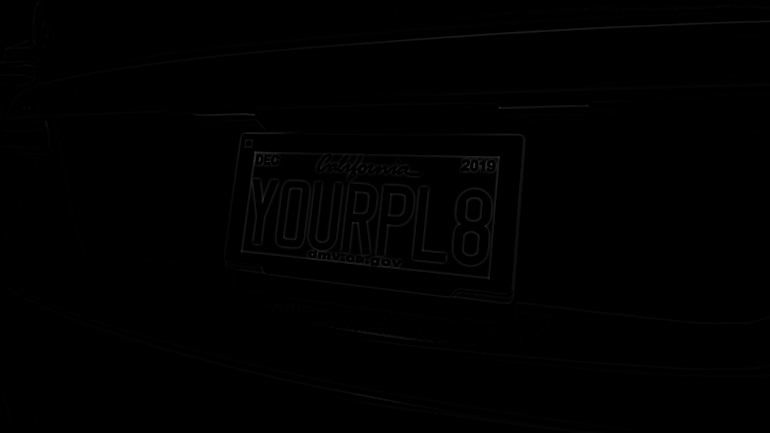
\includegraphics[width=\textwidth]{q1_dog.png}
    \caption{Gaussian Edge Detection (lines are faint - it is not pure black)}
\end{figure}

\begin{figure}[H]
    \centering
    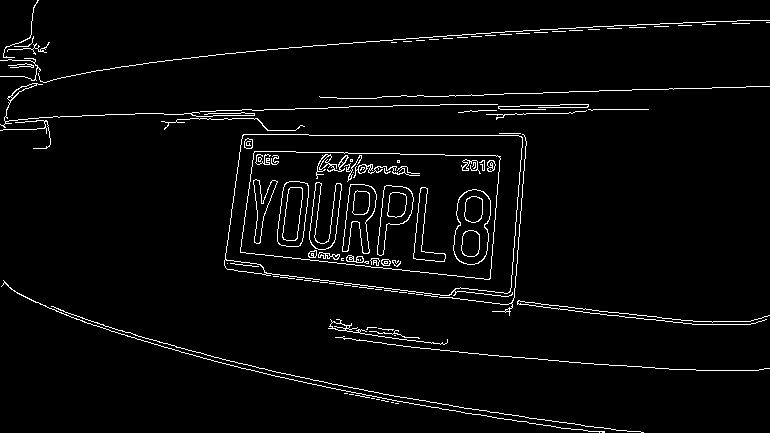
\includegraphics[width=\textwidth]{q1_canny.png}
    \caption{Canny Edge Detection}
\end{figure}

\begin{figure}[H]
    \centering
    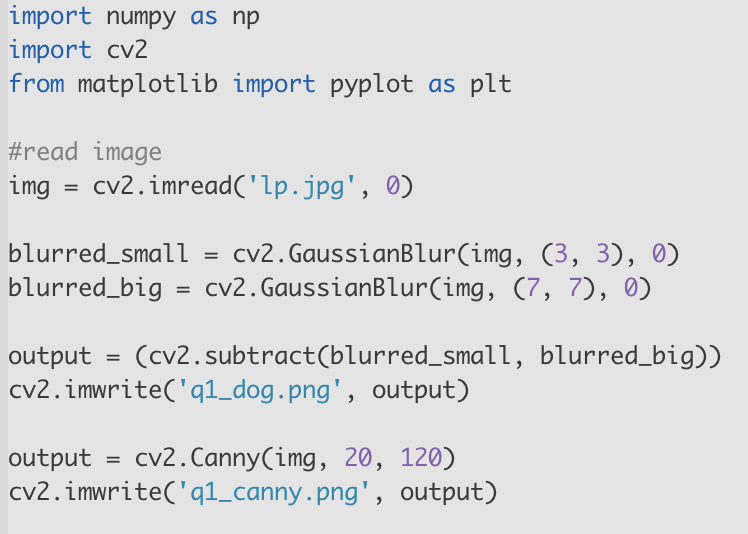
\includegraphics[width=\textwidth]{q1_code.png}
    \caption{Code}
\end{figure}

\subsection{2.}

If we know the scale of our object the DoG method is better since we can fine tune it to only include objects of a certain size by varying the smaller and bigger variances of the kernel.

With the Canny method all we can specify is the lower and upper bounds during the thresholding stage, which is irrelevant of scale of objects.

\subsection{Template Matching}

In the heatmap in Figure 7 we see that the cross correlation template matching produced the highest value in the top left of the image, precisely in the middle of the soccer ball. This is the peak of the heatmap and this shows that this is where the template matching matched the most - therefore, is likely what we are looking for, and in this case it is.
\begin{figure}[H]
    \centering
    \includegraphics[width=\textwidth]{cross_correlate.png}
    \caption{Cross Correlation Heatmap}
\end{figure}

\begin{figure}[H]
    \centering
    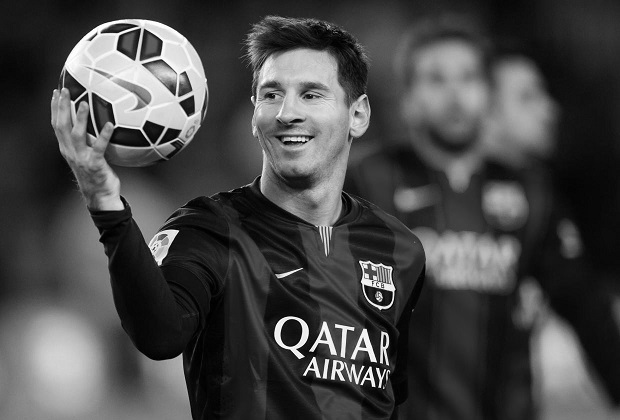
\includegraphics[width=\textwidth]{messi2.png}
    \caption{Cross Correlation Template Matching Results}
\end{figure}

\begin{figure}[H]
    \centering
    \includegraphics[width=\textwidth]{cv2_template_match.png}
    \caption{OpenCV Template Matching Heatmap}
\end{figure}

\begin{figure}[H]
    \centering
    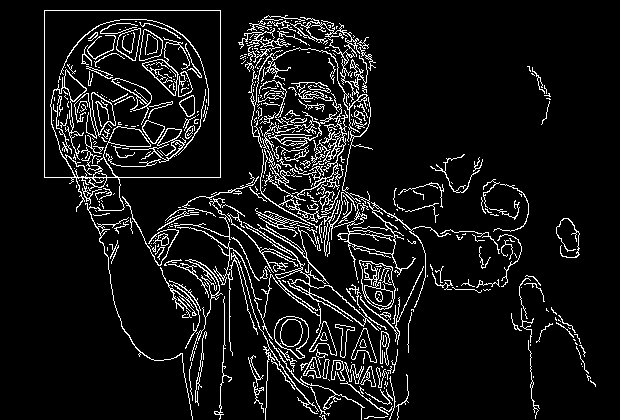
\includegraphics[width=\textwidth]{messi3.png}
    \caption{OpenCV Template Matching Results}
\end{figure}

The biggest difference between my cross correlation implementation and OpenCV's template matching implementation is that the peak of the heatmap is at the top left corner of the soccer ball rather than the center of the soccer ball as in my implementation.

A naive, and simple solution for template matching when the scale of the template is unknown, is to iterate the scale of the template, and simply try many scales, and eventually, you will likely find the object for which you are searching. See the implementation below. There are many matches at different scale values, but we see that eventually the soccer ball is found when the loop reaches the correct scale. 
\begin{figure}[H]
    \centering
    \includegraphics[width=\textwidth]{messi_4.png}
    \caption{Unknown Scale Template Matching Results}
\end{figure}

\begin{figure}[H]
    \centering
    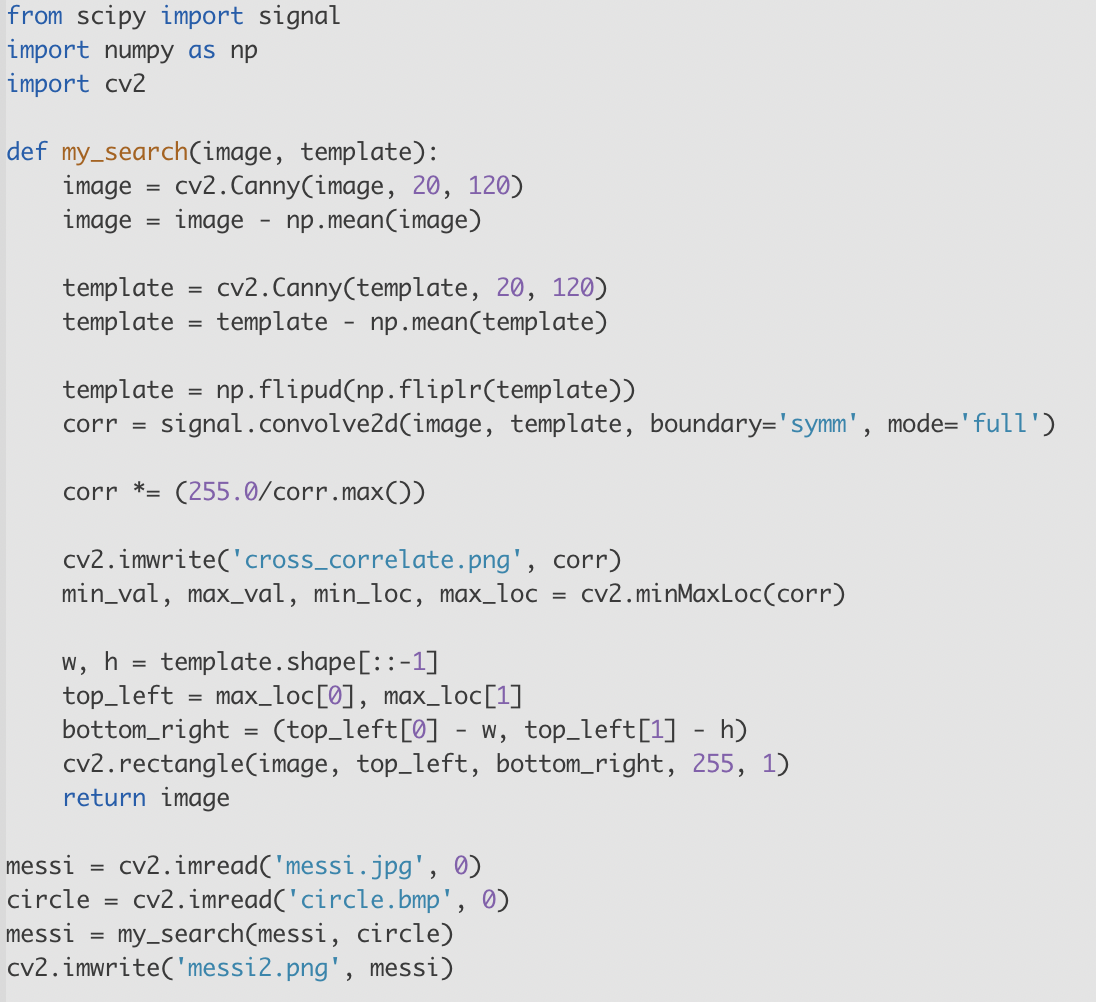
\includegraphics[width=\textwidth]{q2_1_code.png}
    \caption{Cross Correlation Code}
\end{figure}

\begin{figure}[H]
    \centering
    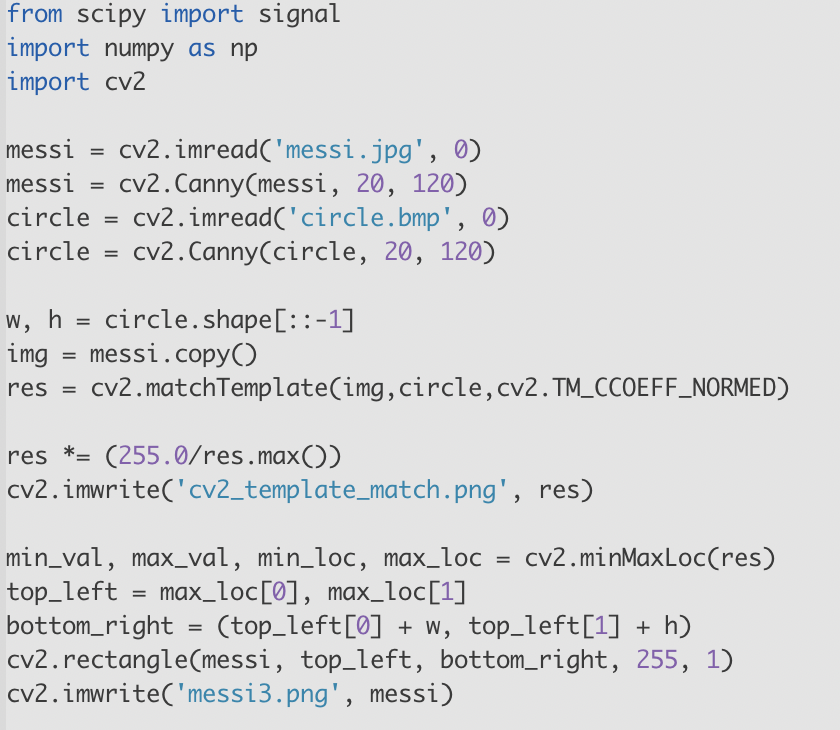
\includegraphics[width=\textwidth]{q2_2_code.png}
    \caption{Open CV Template Matching Code}
\end{figure}

\begin{figure}[H]
    \centering
    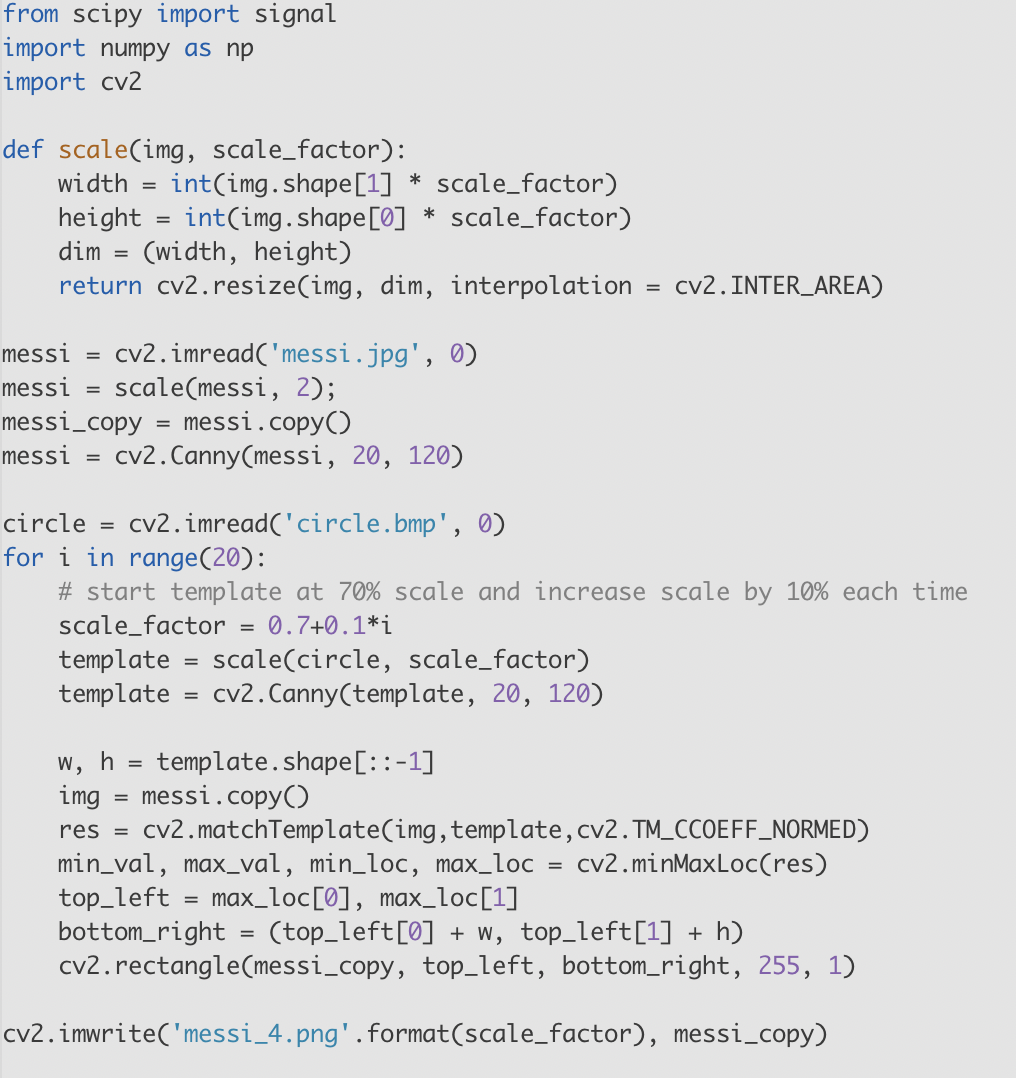
\includegraphics[width=\textwidth]{q2_3_code.png}
    \caption{Unknown Scale Template Matching Code}
\end{figure}




\end{document}

